% --------------------------------------------------------------
% This is all preamble stuff that you don't have to worry about.
% Head down to where it says "Start here"
% --------------------------------------------------------------

\documentclass[12pt]{article}

\usepackage[margin=1in]{geometry}
\usepackage{amsmath,amsthm,amssymb}
\usepackage{graphicx} %This allows to include eps figures
\usepackage{subcaption}
\usepackage[section]{placeins}
\usepackage{layout}
\usepackage{etoolbox}
\usepackage{mathabx}
\usepackage{animate}
\usepackage{array}
% This is to include code
\usepackage{listings}
\usepackage{xcolor}
\definecolor{dkgreen}{rgb}{0,0.6,0}
\definecolor{gray}{rgb}{0.5,0.5,0.5}
\definecolor{mauve}{rgb}{0.58,0,0.82}
\lstdefinestyle{Python}{
    language        = Python,
    basicstyle      = \ttfamily,
    keywordstyle    = \color{blue},
    keywordstyle    = [2] \color{teal}, % just to check that it works
    stringstyle     = \color{green},
    commentstyle    = \color{red}\ttfamily
}

\newenvironment{conditions}
  {\par\vspace{\abovedisplayskip}\noindent\begin{tabular}{>{$}l<{$} @{${}={}$} l}}
  {\end{tabular}\par\vspace{\belowdisplayskip}}

\newcommand{\N}{\mathbb{N}}
\newcommand{\Z}{\mathbb{Z}}

\newenvironment{theorem}[2][Theorem]{\begin{trivlist}
\item[\hskip \labelsep {\bfseries #1}\hskip \labelsep {\bfseries #2.}]}{\end{trivlist}}
\newenvironment{lemma}[2][Lemma]{\begin{trivlist}
\item[\hskip \labelsep {\bfseries #1}\hskip \labelsep {\bfseries #2.}]}{\end{trivlist}}
\newenvironment{exercise}[2][Exercise]{\begin{trivlist}
\item[\hskip \labelsep {\bfseries #1}\hskip \labelsep {\bfseries #2.}]}{\end{trivlist}}
\newenvironment{reflection}[2][Reflection]{\begin{trivlist}
\item[\hskip \labelsep {\bfseries #1}\hskip \labelsep {\bfseries #2.}]}{\end{trivlist}}
\newenvironment{proposition}[2][Proposition]{\begin{trivlist}
\item[\hskip \labelsep {\bfseries #1}\hskip \labelsep {\bfseries #2.}]}{\end{trivlist}}
\newenvironment{corollary}[2][Corollary]{\begin{trivlist}
\item[\hskip \labelsep {\bfseries #1}\hskip \labelsep {\bfseries #2.}]}{\end{trivlist}}



\begin{document}

% --------------------------------------------------------------
%                         Start here
% --------------------------------------------------------------

%\renewcommand{\qedsymbol}{\filledbox}

\title{Assignment 4}%replace X with the appropriate number
\author{Nalet Meinen and Pascal Wyss\\ %replace with your name
Finite Element Analysis I
}
\maketitle

\begin{figure}[!htb]
  \centering
  \vspace*{1cm}
  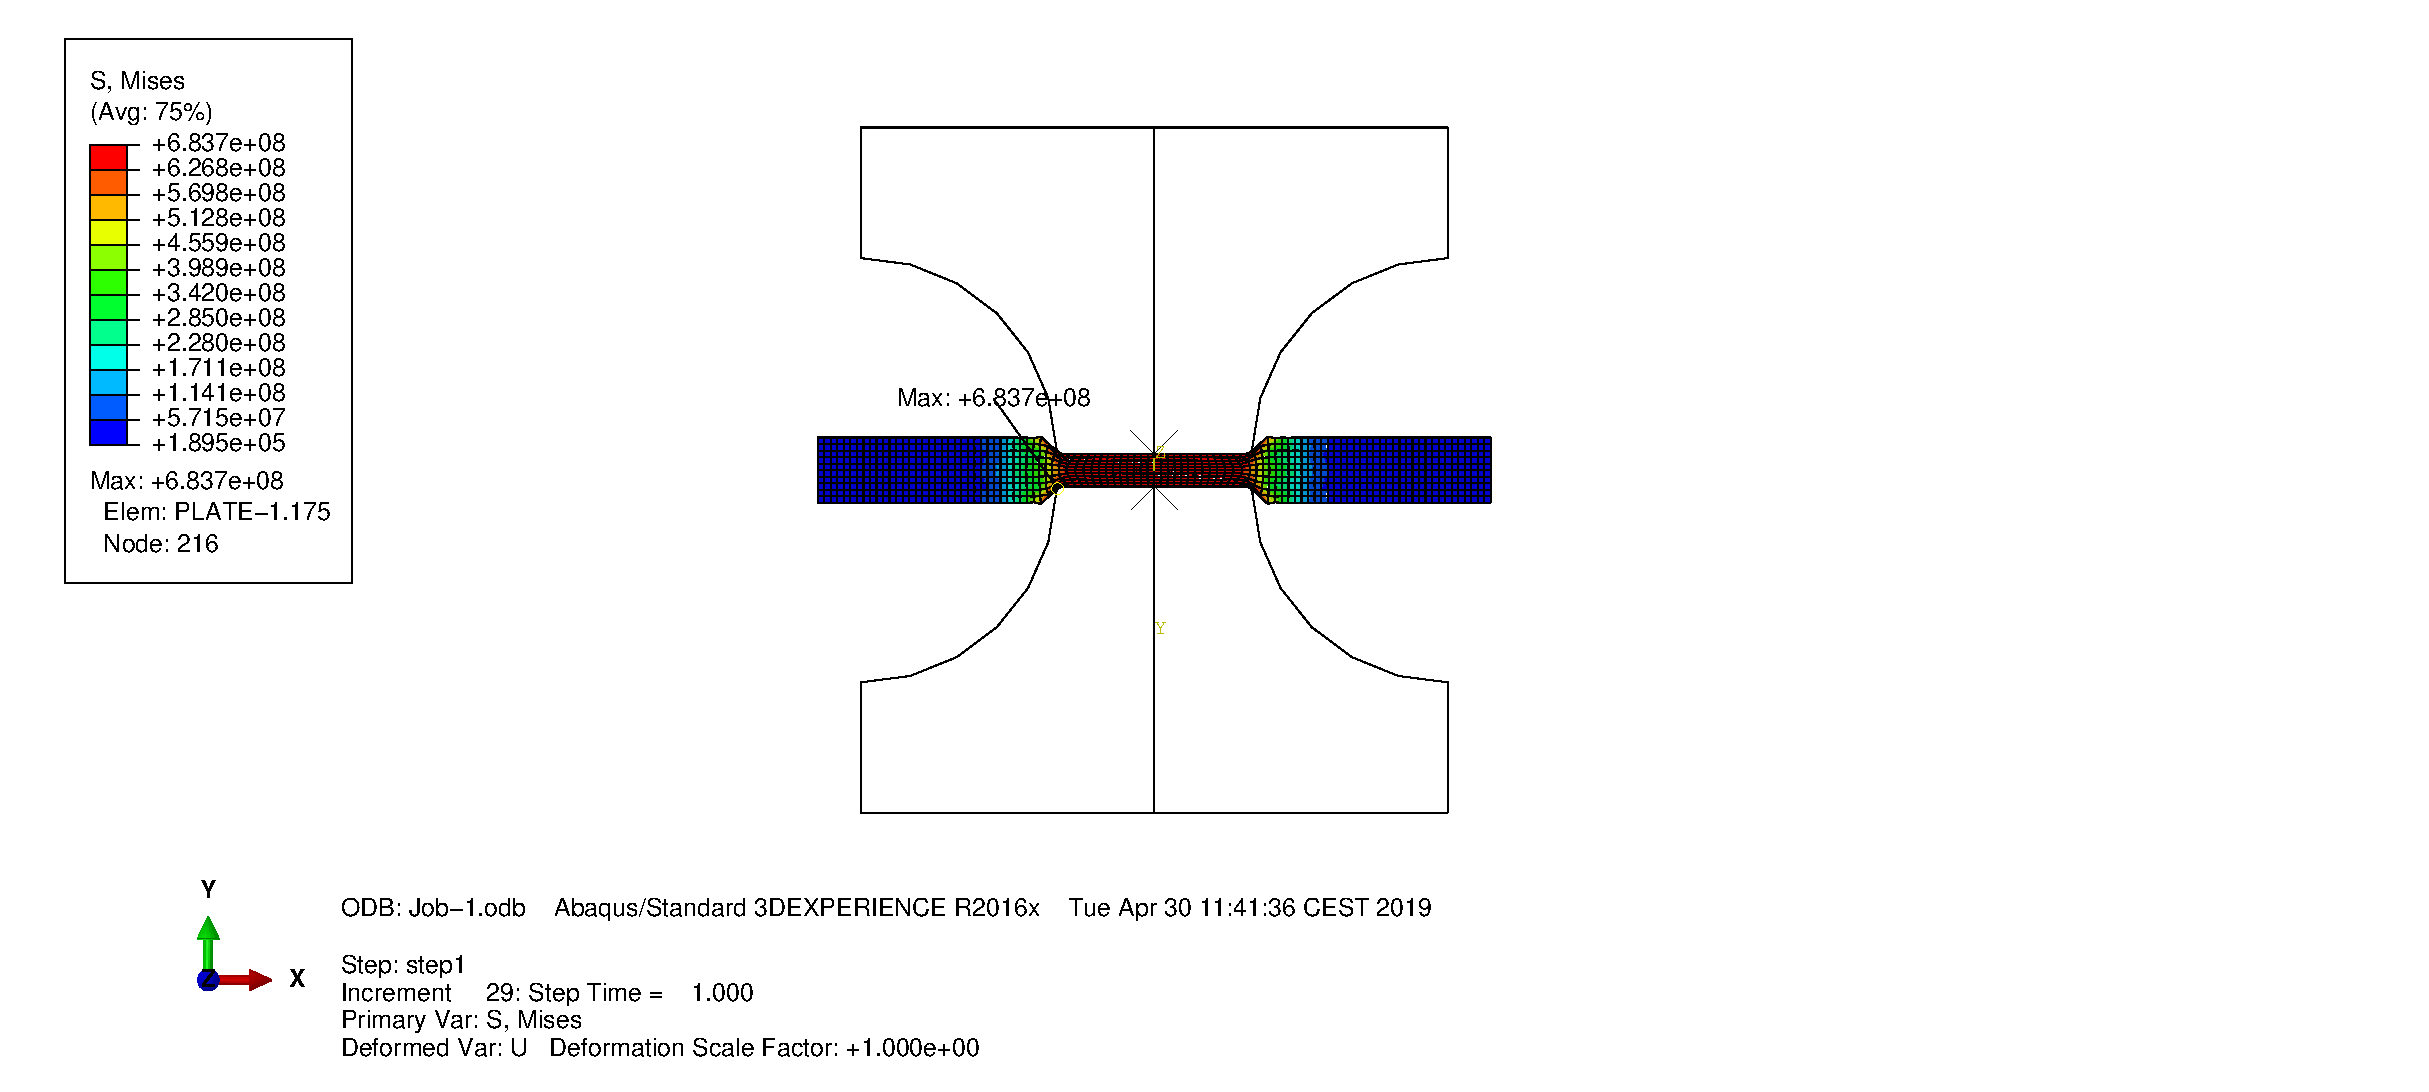
\includegraphics[trim={10cm 4cm 12cm 1cm},clip,width=1.0\linewidth]{pics/titelbild}
\end{figure}

\newpage

\section*{Abstract}
In this assignment we examine the behaviour of a beam after being subjected to an impulse.
The goal is to extract the resonance frequency of the beam with the given dimensions and material coefficients.


% \begin{figure}[!htb]
%   \centering
%   \animategraphics[autoplay,loop,width=0.8\linewidth,trim={1mm 1mm 1mm 1mm}]{4}{pics/out/ani-}{1}{62}
%   \caption{Animation of frequency on beam}
% \end{figure}

\tableofcontents
\pagebreak
\section{Introduction}
The goal of this assignment is to examine contact forces and the behaviour of a 
certain material under compression.
The plate (some kind of metal / aluminium) is being squeezed by a press stamp. Due to 
the given material characteristics,
certain forces are excerted on the surface of the press and the plate. 
Using this forces, and the respective deformation, we can reverse engineer 
the material characteristics and compare it with the analytical solutions.


\begin{figure}[!htb]
  \centering
  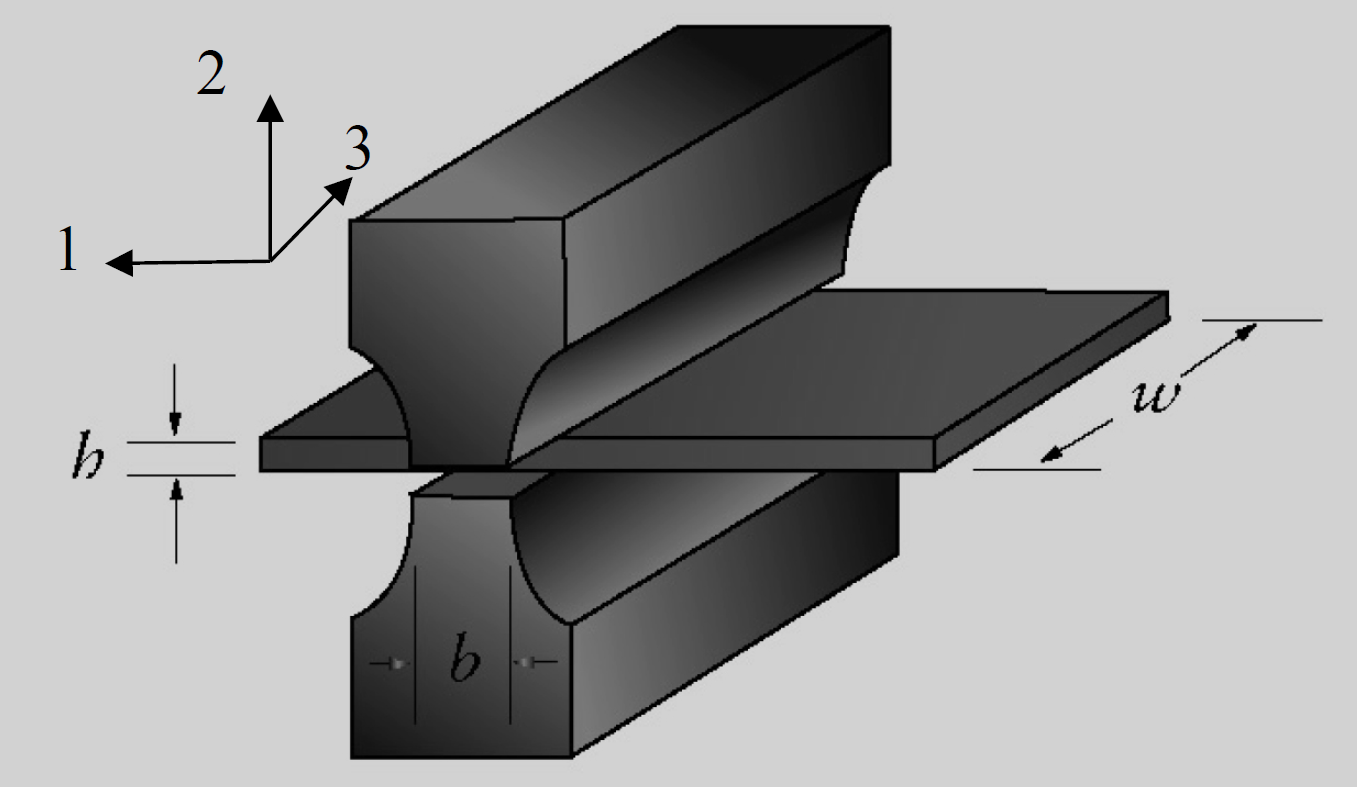
\includegraphics[width=0.6\linewidth]{pics/shematics}
  \caption{Compression of the aluminum plate}
  \label{fig:1}
\end{figure}
\newpage
\section{Methods}

\subsection{Analytical solution}
In order to ensure the validity of the plane strain assumption, the following relationships have to
be fulfilled:
\begin{equation}\label{eq:1}
  w > 5h, \, w > 5b,\, 2h < b < 4h
\end{equation}
The variables in (\ref{eq:1}) are the same as in Figure \ref{fig:1}

With thouse constraints we assume the following proportions for our model in the analytical solution and later with abaqus:

\begin{equation}\label{eq:2}
  w = 0.2m, b = 0.03m, h = 0.01m
\end{equation}

In our situation, the true stress and true strain are given by:
\begin{equation}\label{eq:3}
  \varepsilon_{1}=-\varepsilon_{2},\,\varepsilon_{2}=ln(\frac{h}{h_{x}}),\,\varepsilon_{3}=0,\,
  \sigma_{1}=0,\,\sigma_{2}=\frac{P}{wb},\,\sigma_{3}=\frac{\sigma_{2}}{2}
\end{equation}
And the equivalent (Mises) stress and strain are defined as:
\begin{equation}\label{eq:4}
  \bar{\varepsilon}=\frac{2}{\sqrt{3}}\varepsilon_{2},\,\bar{\sigma}=\frac{\sqrt{3}}{2}\sigma_{2}
\end{equation}
Plastic deformation of aluminium. In this case, the stress-strain relation is given by:
\begin{equation}\label{eq:5}
  \bar{\varepsilon} = 
  \begin{cases} 
    \frac{\bar{\sigma}}{E} & ,\bar{\sigma} < \sigma_{0} \\
    \frac{\sigma_{0}}{E}+\frac{\sigma_{0}}{B}(\frac{\bar{\sigma}}{\sigma_{0}}-1)^{n} & ,\bar{\sigma} >= \sigma_{0}
  \end{cases}
\end{equation}
Where:
\begin{conditions}
  E           & 70 GPa \\
  \sigma_{0}  & 220 MPa \\   
  B           & 3 GPa \\
  n           & 3.2 \\
  v           & 0.3
\end{conditions}
\noindent Using our values for $\bar{\sigma} >= \sigma_{0}$ in equation \ref{eq:5}:
\begin{equation}
  \frac{2}{\sqrt{3}}ln(\frac{200 \cdot 10^{-3}m}{h_{x}}) = \frac{220 \cdot 10^6 Pa}{70 \cdot 10^9 Pa}+\frac{220 \cdot 10^6 Pa}{3 \cdot 10^9 Pa}(\frac{\bar{\sigma}}{220 \cdot 10^6 Pa}-1)^{3.2}
\end{equation}
Or more simple:
\begin{equation}
  (\sqrt[n]{(\bar{\varepsilon}-\frac{\sigma_{0}}{E})\frac{B}{\sigma_{0}}}+1)\sigma_{0}=\bar{\sigma}
\end{equation}

\begin{figure}[!htb]
  \centering
  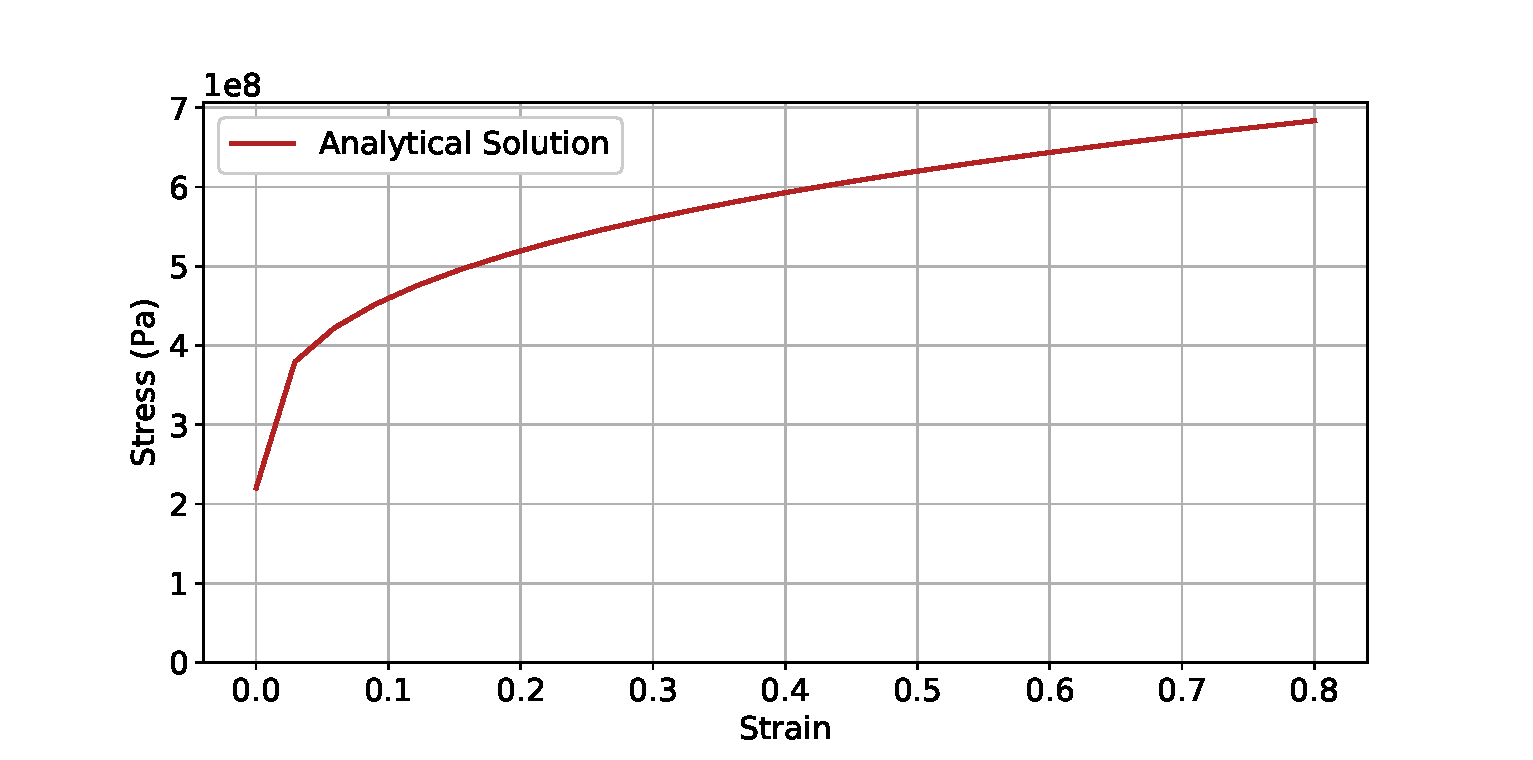
\includegraphics[width=0.9\linewidth]{pics/analytical}
  \caption{Result of the analytical calculations}
  \label{fig:2}
\end{figure}

In the end we used the calculated vales for the platisity in abaqus.

\newpage
\subsection{Plain Stress Compression Test in Abacus}

We created a model with CPS4R mesh type. Based on the last assignments, the reduced integration
gave us the best result, so we stick with that.

\begin{figure}[!htb]
  \centering
  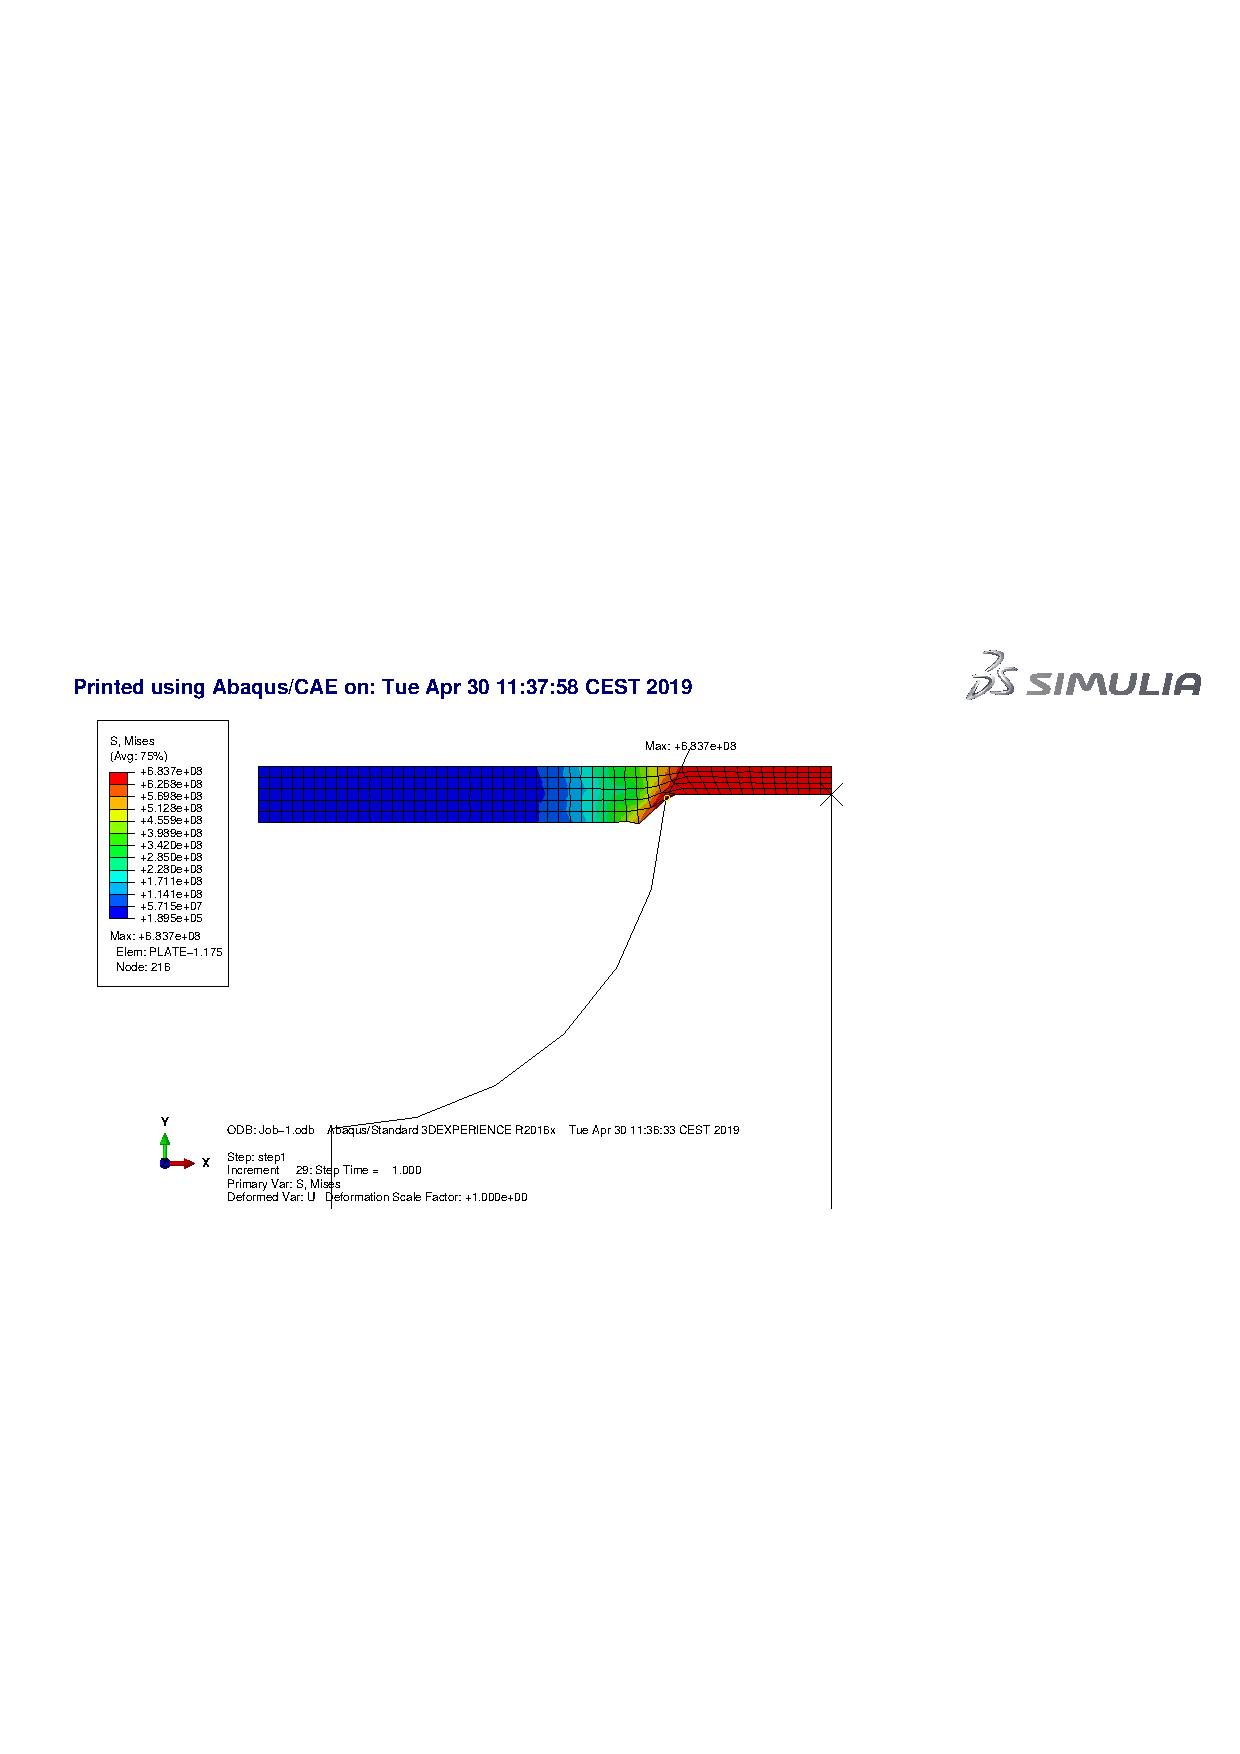
\includegraphics[width=0.9\linewidth]{pics/node_to_node_no_sliding}
  \caption{Node to node with no sliding}
  \label{fig:2}
\end{figure}

\begin{figure}[!htb]
  \centering
  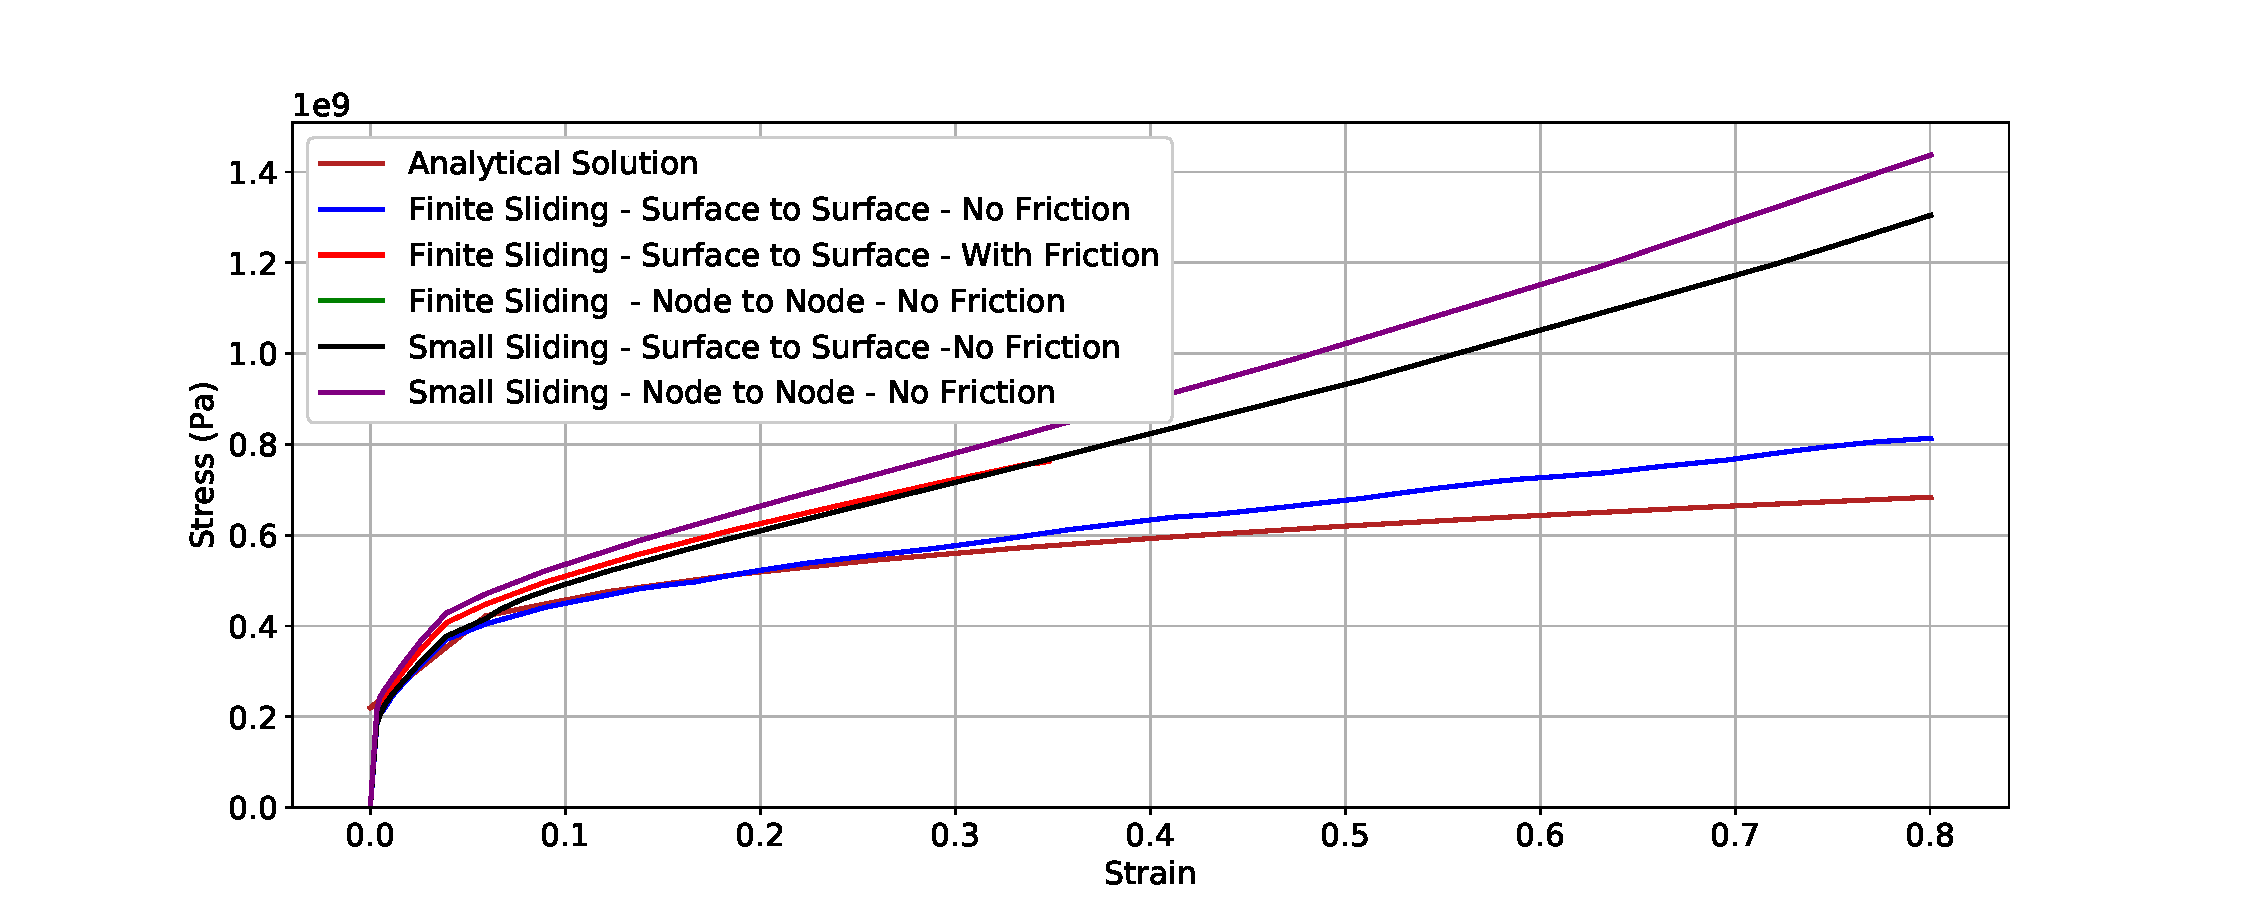
\includegraphics[width=0.9\linewidth]{pics/analytical_compared}
  \caption{Result of the analytical calculations compared with the results form abacus}
  \label{fig:2}
\end{figure}


\pagebreak
\section{Results and Discussion}

In the submodel with the 1mm fillet, we observe an evenly distributed stress pattern. Also,
the maximum value for stress has decreased by about 50 MPa. From a mechanical point of view, 
the round corner offers a smoother distribution of internal stresses because the lines of 
forces in a material are not interrupted. However, the maximum stress is still the yield 
stress of our material, we still expect it to deform.

\pagebreak
\begin{thebibliography}{9}
  \bibitem{latexcompanion} 
  Michel Goossens, Frank Mittelbach, and Alexander Samarin. 
  \textit{The \LaTeX\ Companion}. 
  Addison-Wesley, Reading, Massachusetts, 1993.
\end{thebibliography}


\end{document}